\chapter{Revisão Bibliográfica}
%\markboth{\thechapter ~~~ Revisão Bibliográfica}{}
%\label{revBib}

Esta monografia pretende validar estratégias de controle em um manipulador robótico 
por meio da técnica \textit{Hardware in the Loop} (HIL). Por esse motivo, este capítulo 
aborda uma breve revisão dos principais aspectos que envolvem o tema proposto: manipuladores 
robóticos, sistemas de controle e HIL. Por clareza, esses tópicos são apresentados em seções 
distintas.


\section{Manipuladores Robóticos}
\markright{\thesection ~~~ Manipuladores Robóticos}
%\label{manipRob}

Um manipulador robótico pode ser definido como um mecanismo reprogramável e multifuncional
que é desenvolvido para mover materiais, peças e ferramentas \cite{Murphy:2000:IAR:517685}. 
Mecanismo este que é composto por elos e juntas mecânicas. Apesar disso, o manipulador não pode ser 
visto apenas como uma série de elos (ou \textit{links}) em cascata. Para \citeonline{Spong}, 
o manipulador robótico é composto por um braço mecânico, pela ferramenta no fim do braço 
(também chamada ferramenta de trabalho), pela fonte de energia externa, pelos sensores 
externos e internos, pela interface de comunicação com o sistema e pelo controle do microcontrolador.

Na construção do manipulador, os elos são conectados por meio de juntas formando a cadeia 
cinemática. Segundo \citeonline{paul1981robot}, ao incorporar coordenadas em cada elo do manipulador, 
usando transformação homogênea, é possível descrever a posição relativa e a orientação entre elas.
A transformação homogênea trata-se da transformação de coordenadas que descreve a posição e a orientação 
do eixo da ferramenta de trabalho em relação à base (eixo $0$) \cite{siciliano}.

As juntas podem ser tanto de revolução quanto prismáticas \cite{paul1981robot}. As juntas de revolução
são aquelas que permitem um movimento de rotação entre um elo e outro. Por outro lado,
as prismáticas são as que possibilitam apenas um movimento linear entre os elos.

A forma geométrica para se classificar os manipuladores é dada pela disposição das juntas 
na cadeia cinemática. Segundo \citeonline{Spong}, a maioria dos manipuladores se 
enquadra em uma das categorias a seguir (em que R corresponde a uma junta de revolução 
e P uma junta prismática): articulada (RRR), esférica (RRP), SCARA (RRP), cilíndrica 
(RPP), ou Cartesiana (PPP).

O grau de liberdade (DOF - \textit{degree-of-freedom}) é um parâmetro fundamental para 
a configuração espacial do manipulador robótico. É esse parâmetro que define qual a dimensão do 
espaço de configuração, ou seja, um manipulador possui \textit{n} graus de liberdade caso sua 
configuração seja minimamente especificada por \textit{n} parâmetros \cite{Spong}. Para 
\citeonline{Spong}, a maioria dos manipuladores industriais atualmente possuem seis 
ou menos graus de liberdade.

É importante ressaltar que a planta utilizada neste trabalho é um manipulador com três juntas
revolutas. O manipulador real, possui outras duas juntas, uma para o punho e outra para a garra, entretanto estas 
foram desconsideradas para a modelagem e para o controle. Esse manipulador está representado na \autoref{fig:manipuladorRRR} e 
também é conhecido na literatura como manipulador de cotovelos (\textit{elbow manipulator}), articulado, revoluto, 
antropomórfico (\textit{anthropomorphic manipulator}) ou manipulador RRR.

\begin{figure}[ht]
  \centering
  \caption{Planta utilizada - manipulador de três juntas revolutas}
  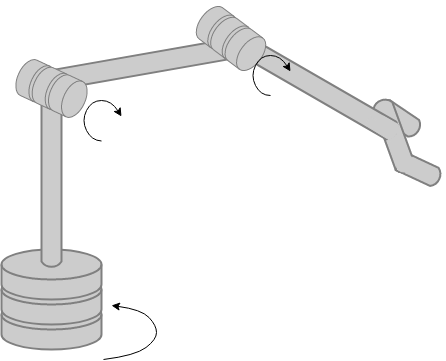
\includegraphics[width = 0.5\columnwidth]{Imagens/manipulador.png}
  \fonte{Do autor}
  \label{fig:manipuladorRRR} 
\end{figure}

\section{Sistemas de Controle}
\markright{\thesection ~~~ Sistemas de Controle}
%\label{manipRob}

Segundo \citeonline{Phillips}, um controlador é necessário em uma planta 
para processar um sinal de erro de forma a atender certas especificações pré-definidas. 
Esse sinal de erro é dado pela diferença entre a resposta do sistema, 
determinada por um sensor, e a trajetória desejada. Dentre as especificações mais 
comuns em controle de sistemas dinâmicos lineares estão: rejeição do 
distúrbio, erro em estado estacionário e a resposta transiente \cite{Ogata}.

As variedades de controle se dão conforme os tipos de sinais existentes. Sinais 
analógicos são aqueles que apresentam valor em qualquer instante de tempo, os 
sinais discretos apresentam valores em instantes múltiplos do tempo de amostragem, e 
por fim, os sinais digitais são aqueles amostrados no tempo tendo sua 
amplitude representada por um número limitado de \textit{bits}, ou seja, a amplitude 
sofre o efeito da quantização \cite{Castrucci}. Geralmente, no projeto de controladores
digitais, primeiro é realizado o projeto do controlador analógico, o qual é convertido, 
então, em digital para execução computacional. Por outro lado, existem também 
metodologias para a síntese direta de controladores digitais, as quais podem fornecer 
melhores resultados quando comparadas ao método indireto. Todavia, essas últimas são menos utilizadas.

Nos dias atuais, o controlador mais utilizado na indústria é o controlador PID. 
Segundo \citeonline{Ogata}, mais da metade dos controladores industriais empregam
o controle PID ou variantes. O seu sucesso está ligado diretamente a sua 
concepção robusta e sua aplicabilidade geral a maioria dos sistemas. O seu nome 
advém das componentes que definem a lei de controle, dada na Equação \eqref{eq:pid}, a qual é composta
pelas ações proporcional, integradora e derivativa \cite{Castrucci}:

\begin{equation}
  \begin{gathered}
    u(t) = K_p\left(e(t)+\frac{1}{T_i}\int_{0}^{t}e(d\tau)d\tau+T_d\frac{de(t)}{dt}\right)
  \end{gathered}
  \label{eq:pid}
\end{equation}
com:

\begin{itemize}
 \item \textit{u(t)}: sinal de saída do controlador, ou variável manipulada;
 \item \textit{e(t)}: sinal de entrada do controlador, ou erro entre a resposta do sistema e o sinal de referência;
 \item $K_p$, $T_i$, $T_d$: parâmetros de ajustes do PID.
\end{itemize}

No escopo desta monografia, o controle PID será utilizado em conjunto com a técnica HIL apresentada 
na próxima subseção. Apesar disso, outras técnicas de controle podem ser igualmente empregadas seguindo 
a metodologia apresentada na monografia.

\section{Técnica \textit{Hardware in the Loop (HIL)}}
\markright{\thesection ~~~ Hardware in the Loop}
%\label{hil}

A idéia básica da técnica HIL é a inclusão de 
uma parte do \textit{hardware} real no loop de simulação durante o desenvolvimento 
do sistema \cite{Bacic}. Isto é, a técnica consiste em inserir um dispositivo físico 
na malha de controle de uma simulação. Nessa técnica, uma parte do sistema é integrada 
a uma outra parte que está sendo simulada em tempo real \cite{Abourida}.

Os primeiros usos da técnica HIL estão relacionados com 
as simulações de vôo \cite{Isermann}. Utilizando essa técnica, a NASA realizou simulações de alta 
fidelidade para o desenvolvimento de tecnologias de aeronaves altamente manobráveis \cite{Evans}. 
Outras aplicações dessa técnica vieram posteriormente com os testes dinâmicos de componentes 
de veículos, como, por exemplo, suspensão e corpo do carro \cite{Isermann}.

Para \citeonline{Abourida}, a técnica \textit{Hardware-in-the-Loop} (HIL) é fundamental
para simulações em tempo real; não para simular o sistema completo em tempo real, mas sim
para conectar uma parte do sistema a um modelo digital em tempo real. Além disso, essa técnica
de simulação tem como desafio o alcance da precisão de um modelo aceitável com um tempo de simulação 
digital viável \cite{Abourida}. Isso porque alguns sistemas (aqueles altamente não-lineares)
precisam de uma frequência de amostragem muito alta para alcançarem uma precisão aceitável.

A técnica HIL será utilizada nesta monografia através do uso de um computador de placa única
de tamanho reduzido (\textit{Raspberry}). A \textit{Raspberry} representa o \textit{Hardware} 
do método, e ela será inserida na malha de controle após a etapa de modelagem e controle no 
ambiente simulado.

\clearpage